%\addtolength{\oddsidemargin}{-.875in}
%\addtolength{\evensidemargin}{-.875in}
%\addtolength{\topmargin}{-.525in}
%\addtolength{\textwidth}{1.75in}
%\addtolength{\textheight}{1.4in}
%\usepackage{colortbl}
\usepackage{graphicx}

\newenvironment{assgts}{%
\renewcommand \labelenumi {\bfseries \zagrad {\alph {enumi}}}%
\renewcommand \labelenumii {\arabic {enumii}.}%
\begin{enumerate}}{\end{enumerate}}

\newcommand \by [1]{%
  \unskip\nobreak\hfil\penalty50
  \hbox{}\nobreak\hfill{\hbox{\qquad\itshape #1}}\par}
%\newcommand \book[1]{{\slshape #1\/}}
\newcommand \bord [1]{{\bfseries\itshape\selectfont #1\/}}
\newcommand \word [1]{{\itshape #1\/}}
\newcommand \ipaword [1]{[\ipa{#1}]}

% IPA Input
% XeLaTeX has built-in Unicode support, which means IPA input becomes a simple font selection problems.
\newfontfamily \IPAFont{CMUSerif-Roman}
\newcommand \ipa [1]{\bgroup\IPAFont #1\egroup}
\newcommand \bipa [1]{\bgroup\bfseries\IPAFont #1\egroup}
% The following is old LaTeX code.
% \newcommand \ipa [1]{\bgroup\fontencoding{T3}\selectfont\SetUnicodeOption{tipa}#1\egroup}
% \newcommand \bipa [1]{\bgroup\fontencoding{T3}\bfseries\selectfont\SetUnicodeOption{tipa}#1\egroup}
% IPA Input

\let \super \textsuperscript
\newcommand \synt [1]{\L{\textsf{#1}}}
\newcommand \tallstrut {\vrule height 9pt depth 0pt width 0pt}
\newcommand \deepstrut {\vrule height 0pt depth 2pt width 0pt}
\newcommand \placehold {\fbox{\fbox{\quad} \fbox{\quad} \fbox{\quad}}}
\def \hh {\textsuperscript h}
%\let \visiblespace \textvisiblespace
\newcommand \latehta [1]{\quoted{#1\space}}
\newlength\halftext
\halftext=\textwidth \advance \halftext by-50pt \divide \halftext by2
\newcommand \NB {{\ooalign{\hfil\raise.2ex\hbox{\bfseries!}\hfil\crcr\Large$\bigtriangleup$}}}
\ifx \upcase \undefined \newcommand \upcase [1]{\MakeUppercase {#1}}\fi
\newcommand \Upcase {\expandafter \upcase }
\newcommand \Uppcase {\expandafter \expandafter \expandafter \Upcase }
\ifx \zagrat \undefined \newcommand \zagrat [1]{\zagrad{#1.}}\fi
%\newcommand \upsens [2]{\MakeUppercase {#1#2}}
%\newcommand \thead {\expandafter \upsens }
%\let \thead \relax
\mathchardef\nga="223A

\def \6#1(#2,#3,#4,#5,#6,#7){\ifcase #1\or #2\or #3\or #4\or #5\or #6\or #7\fi}

\makeatletter
\def \ps@somestyle {
\let\@oddfoot\@empty
\def\@oddhead{\ifx \N \relax
\textsl {\small \begin{tabular}[t]{@{}l}\nthIOL {\thisth}\ \zagrad{\N{2012}}.\\ \chapname \end{tabular}}\hfill \thepage
\else \thepage \hfill
\textsl {\small \begin{tabular}[t]{r@{}}\R{\nthIOL {\thisth}\ \zagrad{\N{2012}}.}\\ \R{\chapname} \end{tabular}}
\fi }}
%\def \procherk {\hrulefill}
\def \procherk {\leaders \hbox {:}\hfill \kern\z@}
\makeatother

\newcounter {exx}[section]
\newcounter {ex:bundiny}
\ifx \N \undefined
  \let \N \relax
  \let \R \relax
  \let \L \relax
  \newcommand \zagrad [1]{(#1)}
  \def \lr {l}\def \bimapp {rll}
  \newcommand \biline [2]{\addtocounter{exx}{1}\arabic{exx}. & #1. & #2}
  \newcommand \ciline [3]{\addtocounter{exx}{1}\arabic{exx}. & \multicolumn{2}{l}{(#1?)} \\ & #3 & #2.}
  \newcommand \bidyir [2]{\addtocounter{exx}{1}\arabic{exx}. & \bipa{#1.} \\& #2.}
  \newcommand \biriyd [2]{\addtocounter{exx}{1}\arabic{exx}. & #1. \\& \bipa{#2.}}
%  \newcommand \squoted [1]{`#1'}
  \newcommand \squoted [1]{‘#1’}
\else
  \renewcommand \bord [1]{\L{\bfseries\itshape\selectfont #1\/}}
  \renewcommand \bipa [1]{\L{\bgroup\fontencoding{T3}\bfseries\selectfont\SetUnicodeOption{tipa}#1\egroup}}
  \newcommand \zagrad [1]{)#1(}
  \def \lr {r}\def \bimapp {lrl}
  \newcommand \biline [2]{#2 & \R{#1.} & \addtocounter{exx}{1}.\arabic{exx}}
  \newcommand \ciline [3]{&\hfill \R{)#1?(} & \addtocounter{exx}{1}.\arabic{exx}\\ \R{#2.} & #3}
  \newcommand \bidyir [2]{\bipa{#1.} & \addtocounter{exx}{1}.\arabic{exx}\\\hfill \R{#2.}}
  \newcommand \biriyd [2]{\hfill \R{#1.} & \addtocounter{exx}{1}.\arabic{exx}\\\bipa{#2.}}
  \newcommand \squoted [1]{\L{'}#1\L{`}}
\fi
\ifx \zagrad \undefined \fi
\ifx \postpar \undefined \newcommand \postpar {.}\fi
\newcommand \paaS [2]{\bord{#1 paa #2.}}

\newcommand \georow [3]{#1. & \R{#3} & \ipa{[#2]}}

\def \problem {\stepcounter {section}\paragraph{\probword \thesection\ \zagrad{\N{20} \pontword}\postpar }}
\def \solution {\stepcounter {section}\paragraph{\probword \thesection \postpar }}

\newcommand \makepart [1]{\newpage
\thispagestyle{empty}
  \begin{center}%
  {\LARGE \nthIOL {\thisth} \par }
  \vskip 1em{\Large
  \thistown\ \zagrad {\thisland}, \olydates {30}{\Julyname}{3}{\Auguname}{2012}
  \par }
%  \vskip 1em{\begin{tabular}[t]{c}\Large
%  \thistown\ (\thisland), \olydates {30}{\Julyname}{3}{\Auguname}{2012}
%  \end{tabular}\par }
  \vskip 1em{\large #1}\end{center}\par \vskip .5em
  \def \chapname {#1}\setcounter {section}0\setcounter {page}1}

\newcount \uuq
\newcount \uur
\newcount \uux
\newcount \uuy
\newcommand \nuu [1]{\ifcase #1\or telu\or talu\or yepoko\fi}
\newcommand \tuu [1]{\uux=#1\advance\uux by-2
  \ifnum 18<\uux tokapu yepoko \advance\uux by-18
  \else \ifnum 12<\uux tokapu talu \advance\uux by-12
  \else \ifnum 6<\uux tokapu \advance\uux by-6
  \fi\fi\fi
  \ifcase \uux\or rurepo\or malapu\or supu\or tokapu\or alapu\or polangipu\or 9\fi}
\newcommand \uu [1]{%
  \ifnum #1<4\nuu {#1}\else
  \uur=#1
  \ifnum 48=\uur tokapu talu\else \ifnum 72=\uur tokapu yepoko\else
    \uuy=#1\divide \uuy by4\uuq=\uuy
    \multiply \uuy by4\advance \uur by-\uuy
    \ifnum0=\uur
      \tuu{\uuq}%
    \else
      \advance \uuq by1\tuu{\uuq}nga \nuu {\uur}%
    \fi
  \fi\fi\fi}
\newcommand \borduu [1]{\bord {\uu {#1}}}
\newcommand \duu [1]{$#1$ & \borduu {#1}}

\begin{document}
\ifx\enumLat\undefined\else\enumLat\fi

\thispagestyle{empty}
\makepart{\probplur {\indicont}}

\pagestyle{somestyle}

%\centerline{\textbf{\regulats}}
%
\regulado. \regulare. \regulami. \towarrant.

\regulaty. \regulatz.\bigskip

\hrule

\problem \givesent {\indiCent {\Dyirbal}}\andtrans {\tothislang}:\medskip \\
%
\begin{tabular}{ll}
\bidyir{bayi yaɽa ŋunɟaymuŋa baŋgu gurugugu biŋgunman}{\dyirbala}\\
\bidyir{balan yabu bimabanɟalŋaymuŋa baŋgul yaɽaŋgu guliŋgu ŋunɟaɲu}{\dyirbalb}\\
\bidyir{balan waymin bambun baŋgu ɟugaŋgu ɟamiman}{\dyirbalc}\\
\bidyir{bala yila wura baŋgul bargandu biŋgundu guniɲu}{\dyirbald}\\
\bidyir{balan malayigara baŋgu garandu biŋgunman}{\dyirbale}\\
\bidyir{bala gurugu baŋgul ŋumaŋgu munduŋgu dimbaɲu}{\dyirbalf}\\
\bidyir{bayi midin baŋgun bimaŋgu malayigaraguninaymuŋagu banɟan}{\dyirbalg}\\
\bidyir{bayi gubimbulu biŋgun baŋgu gurugugu ɟagunman}{\dyirbalh}\\
\bidyir{bala garan baŋgul biɲɟiriɲɟu banɟan}{\dyirbali}\\
\bidyir{balan duŋan baŋgul yiriɲɟilagu guniɲu}{\dyirbalj}\\
\bidyir{bala ɟuga baŋgun yabuŋgu ŋaɟilmuŋagu dimbaɲu}{\dyirbalk}\\
\bidyir{bala diban ɟagiɲ baŋgul gubimbulugu ɟamiŋgu bilmban}{\dyirball}\\
\bidyir{bala garan baŋgun waymindu dibanbilmbalŋaymuŋagu buɽan}{\dyirbalm}\\
\bidyir{balan baŋgay waɽu baŋgun bundiɲɟu ɟagiɲɟu guniɲu}{\dyirbaln}\setcounter {ex:bundiny}{\value {exx}}\\
\bidyir{bayi biɲɟiriɲ biŋgun baŋgul ɲalŋgaŋgu mugurugu buɽan}{\dyirbalo}\\
\bidyir{bayi ŋuma guli baŋgul yaɽaŋgu banɟalmuŋagu munduman}{\dyirbalp}\\
\end{tabular}
%
\begin{assgts}
\item \thoughtE {\Dyirbal}. \nonerror. \babamyth {\Dyirbal}{\quoted {\oldwomen}}. \whatanim? \wheremis?
\item \fordinto {\tothislang}:
\begin{enumerate}\setcounter{enumii}{\value{exx}}
\item\bipa{balan ɲalŋga baŋgul ŋumaŋgu guniymuŋagu bambunman.}
\item\bipa{bala diban bilmbalmuŋa baŋgul biɲɟiriɲɟu guniɲu.}
\item\bipa{bayi bargan baŋgul yaɽaŋgu gubimbuluŋunɟanaymuŋagu banɟan.}
\setcounter{exx}{\value{enumii}}
\end{enumerate}
\item \thremore {\Dyirbal}:
%
\begin{quote}
\bipa{bayimbam} — \bayimbap\if0\bayimbam \else, \bayimbam\fi; \\
\bipa{mugunanɟa} — \auntword\ \zagrad{\mugunanj}; \\
\bipa{muŋga} — \muqgamot.
\end{quote}
%
\fordinto {\tolg {\Dyirbal}}:
\begin{enumerate}\setcounter{enumii}{\value{exx}}
\item \dyirbalq.
\item \dyirbalr.
\item \dyirbals.
\item \dyirbalt.
\end{enumerate}
\end{assgts}
%
\NB \quad \infamily {\Thelg {\Dyirbal}}{\toPNyfam}; \spokNEQL.

\bipa{ŋ} \velarnas.

\bipa{ɲ} \palatnas;
\bipa{ɟ} \samplart {\stopcons\ \zagrad{\like\ \bipa d}}{\bipa{ɲ}}.

\defdeadd. \defwalla. \defpossu. \defstree.
%\defigrog.
%
\by{—\ASname}

\newpage

\problem \mbox{}\medskip\\
%
\begin{tabular}{l|l}
& \R{\lgUndu} \\\hline
\duu{10}\\
\duu{15}\\
\duu{20}\\
\duu{21}\\
\duu{27}\\
\duu{30}\\
\end{tabular}\hfill
\fbox{\L{\borduu 1 < \borduu 3}}\hfill
\begin{tabular}{l|l}
& \R{\lgUndu} \\\hline
\duu{35}\\
\duu{40}\\
\duu{48}\\
\duu{50}\\
\duu{69}\\
\duu{79}\\
\duu{97}\\
\end{tabular}
%
\begin{assgts}
\item \writnums:
\begin{tabular}[t]{l}
\borduu {56},\\
\borduu {57},\\
\borduu {86},\\
\borduu {101}.
\end{tabular}
%
\item \writeout {\lgUndu}: $13$; $66$; $72$; $76$; $95$.
\end{assgts}
%
\NB \quad \infamily {\Thelg{\lgUndu}}{\toTNGfam}. \spokenca{34\,200}{\inPNG}.
%
\by{—\XGname\deepstrut}

\bigskip

\problem \givesent {\inBasque}\andtrans {\tothislang}\chaotict. \pasoreus:
%
\begin{center}
\bord{ahaztu ditut,
ahaztu zaizkit,
ahaztu zaizu,
hurbildu natzaizue,
hurbildu zait,
lagundu ditugu,
lagundu dituzu,
lagundu dute,
lagundu nauzue,
mintzatu natzaizu,
mintzatu gatzaizkizue,
mintzatu zaizkigu,
ukitu ditugu,
ukitu naute}\medskip

\ahazty 23,
\mintzaty 64,
\hurbildy 15,
\mintzaty 12,
\lagundy 46,
\lagundy 51,
\hurbildy 31,
\ukity 46,
\ukity 61,
\lagundy 26,
\lagundy 63,
\mintzaty 45,
\ahazty 16
\end{center}
%
\begin{assgts}
\item \corrcorr.
\item \fordinto {\tolgEus}: \ukity 21, \hurbildy 61.
\item \fordinto {\tothislang}: \bord{lagundu dut}, \bord{hurbildu gatzaizkizu}.
\item \formahat {\tolgEus}. \findtran.
\end{assgts}
%
\by{—\NZname}

\newpage

\problem
\stateopa {\lgTeop}.
\stateope.
\stateopi:\medskip\\
%
\begin{tabular}{\bimapp}
\biline {\teopdata}{\paaS{Ean}{tasu anaa}}\\
\biline {\paani 3{\bonaiana}}{\paaS{Eove}{ani bona iana}}\\
\biline {\teopdatc}{\paaS{Enam}{tasu a beiko}}\\
\biline {\Theman\epaatara {\bonaykae}}{\paaS{A otei}{tara bona kae}}\\
\biline {\Upcase \theboy\teopdate}{\paaS{A visoasi}{asun bona}}\\
\biline {\teopdatf {\tabaqany}}{\paaS{Enaa}{tara a taba’ani}}\\
\biline {\teopdatg}{\paaS{Eam}{baitono e}}\\
\biline {\enaaphee {\oteitomu}{\bonaover}}{\paaS{Enaa}{hee a otei bona overe}}\\
\biline {\Thewoman\teopdati {\tabaqani}}{\paaS{A moon}{hee ameam bona taba’ani}}\\
\biline {\teopdatj}{\paaS{Enaa}{tasu vuan a vasu}}\\
\biline {\teopdatk {\toraaram}}{\paaS{Eori}{asun bona moon bona toraara}}\\
\biline {\teopdatl}{\paaS{Enam}{dao a visoasi bona oraoraa}}\\
\end{tabular}
%
\begin{assgts}
\item \fordinto {\tothislang}:
\begin{enumerate}\setcounter{enumii}{\value{exx}}
\item\paaS{Eam}{ani a overe}
\item\paaS{Ean}{tasu a oraoraa bona kae}
\item\paaS{Eove}{tara ameam}
\setcounter{exx}{\value{enumii}}
\end{enumerate}
\item \fordinto {\tolg {\lgTeop}}:
\begin{enumerate}\setcounter{enumii}{\value{exx}}
\item \teopdatm {\tabaqani}.
\item \teopdatn.
\item \teopdato\ \zagrad{\emph{\litt}\ \withim}.
\item \Upcase \thecerer\heesoasi {\bonaiana}.
\setcounter{exx}{\value{enumii}}
\end{enumerate}
\end{assgts}
%
\stateopo {\lgTeop}.
\stateopu {\lgTeop}\andtrans {\tothislang}.
\stateopy.\medskip\\
%
\begin{tabular}{rll}
\ciline {\teopdaqu}{\Thewoman\teopdatu {\oraoraat}}{\paaS{A moon}{tara bona oraoraa}}\\
\ciline {\Why\teopdaqv}{\paani 4{\tabaqani}}{\paaS{A taba’ani}{ani nam}}\\
\ciline {\Why\didsocry {\theboy}}{\Theman\teopdatw}{\paaS{A visoasi}{tasu a otei bona overe}}\\
\ciline {\teopdaqx}{\enaaphee {\beikoemu}{\bonaekae}}{\paaS{A kae}{hee naa a beiko}}\\
\end{tabular}
%
\begin{assgts}\setcounter{enumi}{2}
\item \fordouta {\tolg {\lgTeop}}:
\begin{enumerate}\setcounter{enumii}{\value{exx}}
\item \zagrad {\Why\offended {\thecerer}?}\ \teopdaty.
\item \zagrad {\Why\teopdaqz?}\ \Upcase \theboy\paaqasun {\bonaiana}{\toraaram}.
\end{enumerate}
\end{assgts}
%
\NB \quad \infamily {\Thelg{\lgTeop}}{\toAustNs}. \spokenca{5\,000}{\inPNG}.
%
\by{—\MKname}

\newpage

\problem \giwordss {\ofRotuma}\andtrans {\tothislang}:\medskip \\
%
\begin{tabular}{l\ifx \N \relax l\else r\fi}
\bord{‘el‘ele} & \R{\qelqele} \\
\bord{‘ele} & \R{\qele} \\
\bord{‘olo} & \R{\qolo} \\
\bord{a‘öf fau} & \R{\aqoffau} \\
%\bord{a‘öf susu} & \R{\aqofsusu} \\
\bord{fäeag ‘u‘u} & \R{\faeagqu} \\
%\bord{fäeag toko} & \R{\faeagtoko} \\
\bord{fau} & \R{\fau} \\
\bord{hạfhạfu} & \R{\hafhafu} \\
\bord{huag ‘el‘ele} & \R{\huagqele} \\
\bord{huag to‘a} & \R{\huagtoqa} \\
\bord{hül hạfu} & \R{\hulhafu\ \zagrad{\hurrican}} \\
\bord{hün kia} & \R{\hunkia} \\
\bord{huli} & \R{\huli} \\
\bord{huni} & \R{\huni} \\
\bord{is ‘ā} & \R{\isqa} \\
\bord{is susu} & \R{\issusu} \\
\bord{lala} & \R{\lala} \\
\bord{maf tiro} & \R{\maftiro} \\
\end{tabular}\hfill
\begin{tabular}{l\ifx \N \relax l\else r\fi}
\bord{mamasa} & \R{\mamasa} \\
\bord{mạtiti} & \R{\matiti} \\
\bord{mạtit mamasa} & \R{\matmamas} \\
\bord{moafmofa} & \R{\moafmofa} \\
\bord{niu} & \R{\niu} \\
\bord{nu‘suar tiro} & \R{\nusutiro} \\
\bord{nu‘sura} & \R{\nusura} \\
\bord{pala} & \R{\pala} \\
\bord{piri} & \R{\piri} \\
\bord{poagpoga = palpala} & \R{\poagpoga} \\
\bord{pogi} & \R{\pogi} \\
\bord{puhrạki} & \R{\puhraki} \\
\bord{pulu} & \R{\pulu} \\
%\bord{rạhu} & \R{\rahu} \\
\bord{kạlu} & \R{\kaluN; \kaluV} \\
\bord{riamrima} & \R{\riamrima} \\
\bord{rū huga} & \R{\ruhuga} \\
\bord{to‘a} & \R{\toqa} \\
%\bord{toko} & \R{\toko} \\
\end{tabular}
%
\begin{assgts}
\item \gyRotuma\andtrans {\tothislang}\chaotict. \corrcorr:\smallskip

\centerline{\bord{‘u‘u, isu, kia, leva, mafa, susu, huga}}
\centerline{\R{\susu, \mafa, \ququ, \leva, \huga, \kia, \isu}}
\item \fordinto {\tothislang}:\smallskip

\centerline{\bord{tiro, poga} \R{\zagrad{\nounword}}\bord{, huag lala, hạf puhrạki, maf pogi = maf pala.}}
\item \fordinto {\tolgRtm}:\smallskip

\centerline{\R{%
%\rahrahu;
\kalkalu;
\niut {\qolo};
\leavpiri;
\pulpulu;
\rima;
\mofa.}}
\item \canttran{\tolgRtm}{\squoted{\faega} \et {\squoted{\aqofi}}}. \whatposs {\tolgRtm}?
\end{assgts}
%
\NB \quad \infamily {\TheRtm}{\toAustNs}. \spokenca {9000}{\inFiji}.

\glotstop {\bord{‘}};
\bord{ạ} \oshiroko;
\aeligatu {\bord{ä}};
\bord{ö} \oeumlaut;
\bord{ü} \ueumlaut.
\longmark {\quoted{\L{\bfseries¯}}}.

\defcopra.
%
\by{—\BIname, \APname}

\vfill
%\hline

\begin{center}
\textbf{\editorsz:} \edinames.\medskip

\textbf{\thistext:} \whowroti.\medskip

\large \goodluck!
\end{center}

\makepart{\soluplur {\indicont}}
%\thispagestyle{empty}
\pagestyle{somestyle}
%
\solution \wordsord\ \fbox{\synt{OSV}}
\zagrad{\synt O: \Ob, \synt S: \Sb, \synt V: \Verb},
\fbox{\synt{NA}}
\zagrad{\synt N: \nounword, \synt A: \adjectif}.

\synt{A $\to$ V} \zagrad{\squoted{\adjeverb {\synt A}}}: \L{\synt A\bipa{-man}}.

\synt{V $\to$ A}:
\begin{tabular}[t]{|l|l|l|}\hline
\synt V & \R{\squoted{\munga {\synt V}}} & \R{\squoted{\ngaymunga {\synt V}{\synt N}}} \\\hline
\bipa{-n} & \bipa{-l-muŋa} & \synt N-\dots\bipa{-l-ŋay-muŋa} \\
\bipa{-ɲu} & \bipa{-y-muŋa} & \synt N-\dots\bipa{-nay-muŋa} \\\hline
\end{tabular}\medskip

\artnomen:\medskip \\
%
\begin{tabular}{|l|l|\lr|}\hline
\synt O & \synt S & \\\hline
\bipa{balan} & \bipa{baŋgun} & \R{\women, \dangerux {\animals}} \\
\bipa{bayi} & \bipa{baŋgul} & \R{\men, \animals} \\
\bipa{bala} & \bipa{baŋgu} & \R{\alltrest} \\\hline
\end{tabular}
\medskip \\

\ergatend
\begin{itemize}
\item \bipa{-ŋgu}, \simotend {\byavowel}\et {\contains {\twosylla}};
\item \bipa{-gu}, \simotend {\byavowel}\et {\contains {\trosylla}};
\item \L{\textbf{-Du}}, \simotend {\byacsant};
\L{\textbf D} \samplart {\stopcons}{\wordlast}.
\end{itemize}
%
\begin{assgts}
\item \bundinye, \mustmyth {\quoted {\oldwoman}}. \theremis {\bipa {baŋgun bundiɲɟu}}{\zagrad{\arabic {ex:bundiny}}}.
\setcounter{exx}{16}
\item \begin{tabular}[t]{ll}
\bidyir{balan ɲalŋga baŋgul ŋumaŋgu guniymuŋagu bambunman}{\dyirbalu}\\
\bidyir{bala diban bilmbalmuŋa baŋgul biɲɟiriɲɟu guniɲu}{\dyirbalv}\\
\bidyir{bayi bargan baŋgul yaɽaŋgu gubimbuluŋunɟanaymuŋagu banɟan}{\dyirbalw}\\
\end{tabular}
\item \begin{tabular}[t]{ll}
\biriyd{\dyirbalq}{bayi yiriɲɟila baŋgul bargandu wuraŋgu buɽan}\\
\biriyd{\dyirbalr}{bala yila baŋgun mugunanɟagu banɟalmuŋagu waɽuman}\\
\biriyd{\dyirbals}{bala muŋga baŋgul midindu ɟagundu ŋaɟin}\\
\biriyd{\dyirbalt}{bayi yaɽa dibandimbanaymuŋa baŋgul bayimbambu guniɲu}\\
\end{tabular}
\end{assgts}

\solution \mbox{}

\begin{tabular}{r|l}
& \R{\lgUndu} \\\hline
\duu{1}\\
\duu{2}\\
\duu{3}\\
\duu{12}\\
\duu{16}\\
\duu{20}\\
\duu{24}\\
\duu{28}\\
\duu{32}\\
\end{tabular}\hfill
\begin{tabular}{l|l}
& \R{\lgUndu} \\\hline
$24$ & \borduu {24}\\
$48=24\times 2$ & \borduu {48}\\
$72=24\times 3$ & \borduu {72}\\
$\alpha \nga \beta := (\alpha-4)+\beta$, & $\alpha\mbox{\bord{-nga}}\ \beta$\\
\quad $\alpha \in \{12,16,20,24,28,32\},$\\
\quad $\beta \in \{1,2,3\}$\\
$\gamma + \delta$, & $\gamma\ \delta$\\
\quad $\gamma = 24k, k \in \{1,2,3\}$,\\
\quad $9\le \delta\le 32, \delta \ne 24$\\
\end{tabular}
%
\begin{assgts}
\item \begin{tabular}[t]{l}
\borduu {56} = $24+32 = 56$,\\
\borduu {57} = $24\times 2+12 \nga 3 = 57$,\\
\borduu {86} = $24\times 3+16 \nga 2 = 86$,\\
\borduu {101} = $24\times 3+32 \nga 1 = 101$.
\end{tabular}
%
\item \begin{tabular}[t]{l}
$13 = 16\nga 1$ = \borduu{13},\\
$66 = 24\times 2+20\nga 2$ = \borduu{66},\\
$72 = 24\times 3$ = \borduu{72},\\
$76 = 24\times 2+28$ = \borduu{76},\\
$95 = 24\times 3+24\nga 3$ = \borduu{95}.
\end{tabular}
\end{assgts}

\solution \mbox{}\smallskip \\
%
\begin{tabular}{|l|l|l|l|l|l|l|}\hline
 & \R{\persnumb1{\Sg}} & \R{\persnumb1{\Pl}}
 & \R{\persnumb2{\Sg}} & \R{\persnumb2{\Pl}}
 & \R{\persnumb3{\Sg}} & \R{\persnumb3{\Pl}}\\\hline
\L{A} & \bord{nau-} & & & & \bord{du-} & \bord{ditu-}\\\hline
\L{B} & \bord{natzai-} & \bord{gatzaizki-} & & & \bord{zai-} & \bord{zaizki-}\\\hline
\L{Z} &\hfill \bord{-t} &\hfill \bord{-gu} &\hfill \bord{-zu} &\hfill \bord{-zue} & &\hfill \bord{-te}\\\hline
%\L{A} & \bord{n-au-} & & & & \bord{d-u-} & \bord{d-it-u-}\\\hline
%\L{B} & \bord{n-at-zai-} & \bord{g-at-zai-zki-} & & & \bord{zai-} & \bord{zai-zki-}\\\hline
%\L{Z} &\hfill \bord{-t} &\hfill \bord{-gu} &\hfill \bord{-zu} &\hfill \bord{-zue} & &\hfill \bord{-te}\\\hline
\end{tabular}
\\
\begin{tabular}{|l|*{4}{\lr|}}\hline
& \L{A} & \L{B} & \L{Z} & \\\hline
\bord{ahaztu} & \multicolumn{2}{c|}{— \R{\ahazt} —} & \R{\who} & \R{\ahaztu} \\\hline
\bord{hurbildu} && \R{\who} & \R{\hurbild} & \R{\hurbildu} \\\hline
\bord{lagundu} & \R{\lagund} && \R{\who} & \R{\lagundu} \\\hline
\bord{mintzatu} && \R{\who} & \R{\mintzat} & \R{\mintzatu} \\\hline
\bord{ukitu} & \R{\ukit} && \R{\who} & \R{\ukitu} \\\hline
\end{tabular}
%
\begin{assgts}
\item \mbox{}\\
\centerline{\begin{tabular}{l\lr}
$\left.\begin{array}{@{}l}\mbox{\bord{ahaztu ditut}} \\\mbox{\bord{ahaztu zaizkit}}\end{array}\right\}$ & \R{\ahazty 16} \\
\bord{ahaztu zaizu} & \R{\ahazty 23} \\
\bord{hurbildu natzaizue} & \R{\hurbildy 15} \\
\bord{hurbildu zait} & \R{\hurbildy 31} \\
\bord{lagundu ditugu} & \R{\lagundy 46} \\
\bord{lagundu dituzu} & \R{\lagundy 26} \\
\end{tabular}\hfill
\begin{tabular}{\ifx \N \relax ll\else lr\fi}
\bord{lagundu dute} & \R{\lagundy 63} \\
\bord{lagundu nauzue} & \R{\lagundy 51} \\
\bord{mintzatu natzaizu} & \R{\mintzaty 12} \\
\bord{mintzatu gatzaizkizue} & \R{\mintzaty 45} \\
\bord{mintzatu zaizkigu} & \R{\mintzaty 64} \\
\bord{ukitu ditugu} & \R{\ukity 46} \\
\bord{ukitu naute} & \R{\ukity 61} \\
\end{tabular}}
\item \ukity 21\ — \bord{ukitu nauzu}, \hurbildy 61\ — \bord{hurbildu zaizkit}.
\item \bord{lagundu dut} — \lagundy 13, \bord{hurbildu gatzaizkizu} — \hurbildy 42.
\item \ahazty 23\ \zagrad{\bord{ahaztu zaizu}} — \bord{ahaztu duzu}.
\end{assgts}

\solution \sestruct: \fbox{\L{\textsf{S} \bord{paa} \textsf{V O [O${}^{'}$]}}}
\zagrad{\synt S: \Sb, \synt V: \Verb, \synt O: \Ob, \synt{O${}^{'}$}: \bis {\Ob}}.\medskip\\
%
\begin{tabular}{|l|\lr|\lr|\lr|}\hline
& \R{\hee} & \R{\dao} & \R{\tasu, \asun} \\\hline
\synt O & \R{\whotom} & \R{\whomcall} & \R{\whom} \\
\synt{O${}^{'}$} & \R{\what} & \R{\whatcall} & \R{\withwhat} \\\hline
\end{tabular}\medskip

\artnomen, \evelbona {\bord{a}}{\bord{bona}}.
\selepron {\persnumb3{\Sg}}{{\bord{e}} \au\ {\bord{bona}}}.

\Perspron:\medskip\\
%
\begin{tabular}{|\lr|l|l|l|l|l|l|}\hline
 & \R{\persnumb1{\Sg}} & \R{\persnumb1{\Pl}}
 & \R{\persnumb2{\Sg}} & \R{\persnumb2{\Pl}}
 & \R{\persnumb3{\Sg}} & \R{\persnumb3{\Pl}}\\\hline
\synt S & \bord{enaa} & \bord{enam} & \bord{ean} & \bord{eam} & \bord{eove} & \bord{eori}\\\hline
\synt O, \synt{O${}^{'}$} & \bord{anaa} & & \bord{vuan} & \bord{ameam} & \bord e, \bord{bona} &\\\hline
\end{tabular}
%
\begin{assgts}
\item
\begin{enumerate}\setcounter{enumii}{12}
\item\paaS{Eam}{ani a overe} — \paani 5{\bonaover}.
\item\paaS{Ean}{tasu a oraoraa bona kae} — \teopdats {\oraoraat}.
\item\paaS{Eove}{tara ameam} — \teopdatt.
\setcounter{exx}{\value{enumii}}
\end{enumerate}
\item
\begin{enumerate}\setcounter{enumii}{\value{exx}}
\item \teopdatm {\tabaqani}. — \paaS{Enam}{hee vuan a taba’ani}
\item \teopdatn. — \paaS{Eove}{dao anaa bona beiko}
\item \teopdato. — \paaS{Enaa}{asun e bona}
\item \Upcase \thecerer\heesoasi {\bonaiana}. — \paaS{A oraoraa}{hee bona visoasi bona iana}
\setcounter{exx}{\value{enumii}}
\end{enumerate}
\end{assgts}
%
\newsavebox{\topics}
\newlength{\topicswide}\newlength{\topicsleft}
\savebox{\topics}{\fbox{\begin{tabular}[t]{r@{ \bord{paa} \textsf V }l@{ $\to$ }r@{ \bord{paa} \textsf V }l}
\synt{\underline S} & \L{\textsf{O [O${}^{'}$]}} & \L{\textsf{\underline S}} & \L{\textsf{O [O${}^{'}$]}} \\
\synt S & \synt{\underline O [O${}^{'}$]} & \synt{\underline O} & \synt{S [O${}^{'}$]} \\
\synt S & \synt{O \underline{O${}^{'}$}} & \synt{\underline {O${}^{'}$}} & \synt{S O} \\
\end{tabular}}}
\settowidth{\topicswide}{\usebox{\topics}}
\topicsleft=\textwidth \advance\topicsleft by-10pt\advance\topicsleft by-\topicswide
\parbox{\topicsleft}{\topicfrt {\bord{a}}.
\pronoffe {\Sb}{\bord{e-}}.
\nounoffe {\Sb}{\bord a}.}\hfill
\parbox{\topicswide}{\usebox{\topics}}
%
\begin{assgts}\setcounter{enumi}{2}
\item
\begin{enumerate}\setcounter{enumii}{\value{exx}}
\item \zagrad {\Why\offended {\thecerer}?}\ \teopdaty.\\— \paaS{A oraoraa}{dao ori bona moon}
\item \zagrad {\Why\teopdaqz?}\ \Upcase \theboy\paaqasun {\bonaiana}{\toraaram}.\\
— \paaS{A toraara}{asun a visoasi bona iana}
\end{enumerate}
\end{assgts}

\newpage

%\solution \twoforms:\medskip \\
\solution \temathes:\medskip \\
%
\begin{tabular}{|l@{ $\to$ }l}
%\longform & \kortform \\\hline
\synt{-VCV} & \synt{-VC} \\
\synt{-VC}\bord u & \synt{-VC} \\
\synt{-VC}\bord i & \synt{-\"VC} \\
\synt{-VC}\bord a & \synt{-V}\bord a\synt C \\
\end{tabular}
\smallskip\
%
\zagrad{\synt V: \vocal, \synt C: \const}.

%\inphrase.
\adjedoub: \L{\bord{‘ele} + \bord{‘ele} $\to$ \bord{‘el‘ele}} \squoted{\qele\ $\times$ 2 = \qelqele}.

\wordsord
\begin{itemize}
\item \fbox{\synt{N$_1$ N$_2$}} \zagrad{\synt{N$_1$}: \attribum, \synt{N$_2$}: \attribut};
\item \fbox{\synt{N A}} \zagrad{\alsomean \squoted {\hewhohas {\synt A}{\synt N}}:
\bord{huag ‘el‘ele} \squoted{\huga\ + \qelqele\ = \huagqele}};
\item \fbox{\synt{V O}} \zagrad{\nounverb:
\bord{a‘öf fau} \squoted{\aqofi\ + \fau\ = \aqoffau},
\bord{hül hạfu} \squoted{\huli\ + \hafu\ = \hulhafu\ \zagrad{\hurrican}}}.
\end{itemize}

\begin{assgts}
\item
\bord{‘u‘u} — \ququ,
\bord{isu} — \isu,
\bord{kia} — \kia,
\bord{leva} — \leva,
\bord{mafa} — \mafa,
\bord{susu} — \susu,
\bord{huga} — \huga.
\item
\bord{tiro} — \tiro,\\
\bord{poga} — \poga,\\
\bord{huag lala} — \huaglala,\\
\bord{hạf puhrạki} — \hafpraki,\\
\bord{maf pogi = maf pala} — \mafpogi.
\item
%\rahrahu\ — \bord{rạhrạhu};
\kalkalu\ — \bord{kạlkạlu};
\niut {\qolo} — \bord{‘ol niu};
\leavpiri\ — \bord{leav pirpiri};
\pulpulu\ — \bord{pulpulu};
\rima\ — \bord{rima};
\mofa\ — \bord{mofa}.
\item
\begin{itemize}
\item \faega: \bord{fäega} \zagrad{\au\ \bord{fäeaga, fäeagu}}.
\item \aqofi: \bord{a‘ofi} \zagrad{\au\ \bord{a‘öfi, a‘öfö, a‘öfu, a‘öfü, a‘ofü}}.
\end{itemize}
\end{assgts}

\makepart {\enquetex}
\enqueten:\vskip 1in

\enquetep:\vskip 1in

\enquetea?\vskip 1in

\enqueteb?\vskip 1in

\enquetec {\seemhard}?\vskip 1in

\enquetec {\seemeasy}?

\makepart{\probsing {\teamcont}}
%\thispagestyle{empty}
\pagestyle{somestyle}

\giveland {\N{57}}:

% geo57Lao.pdf
% Things changed because of XeLaTeX
% It just works and I don't know the reason.
% Good luck!
\L{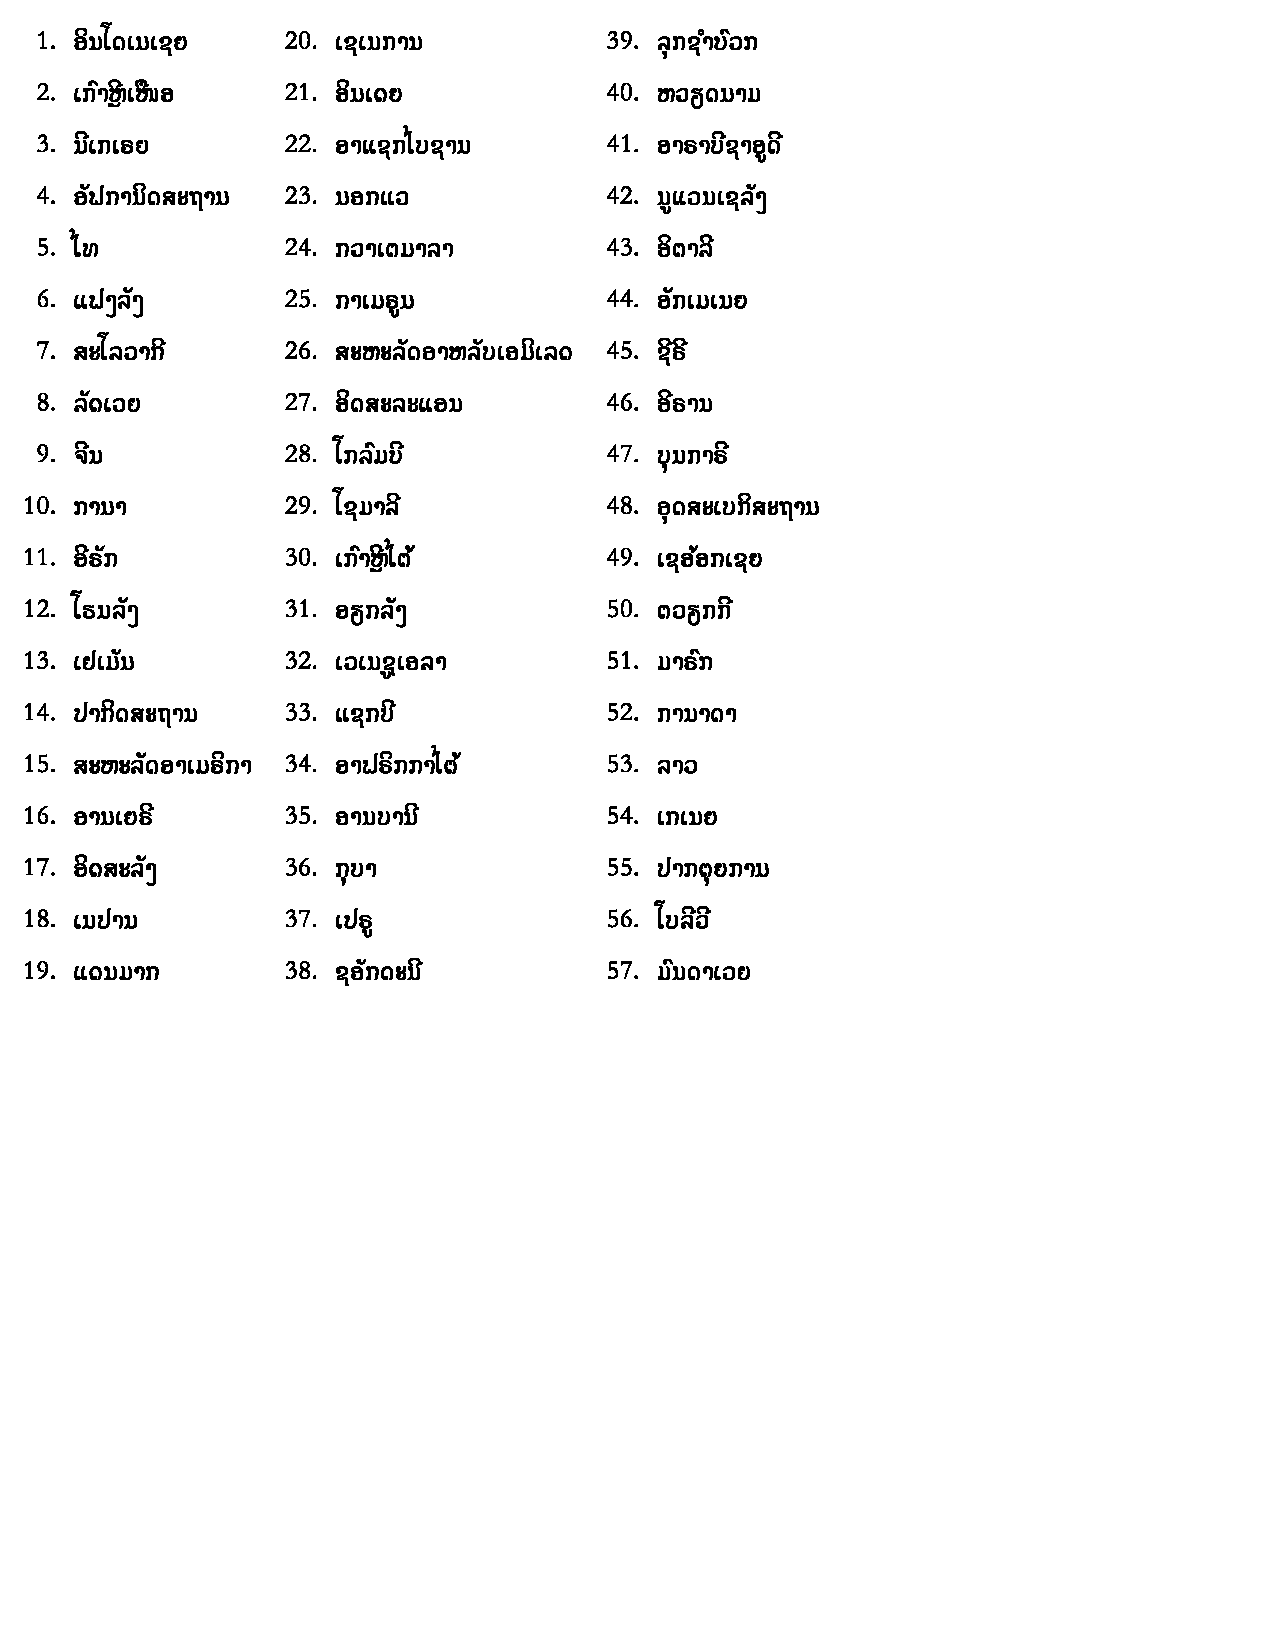
\includegraphics[trim = 0 320 320 0]{geo57Lao.pdf}}
%\L{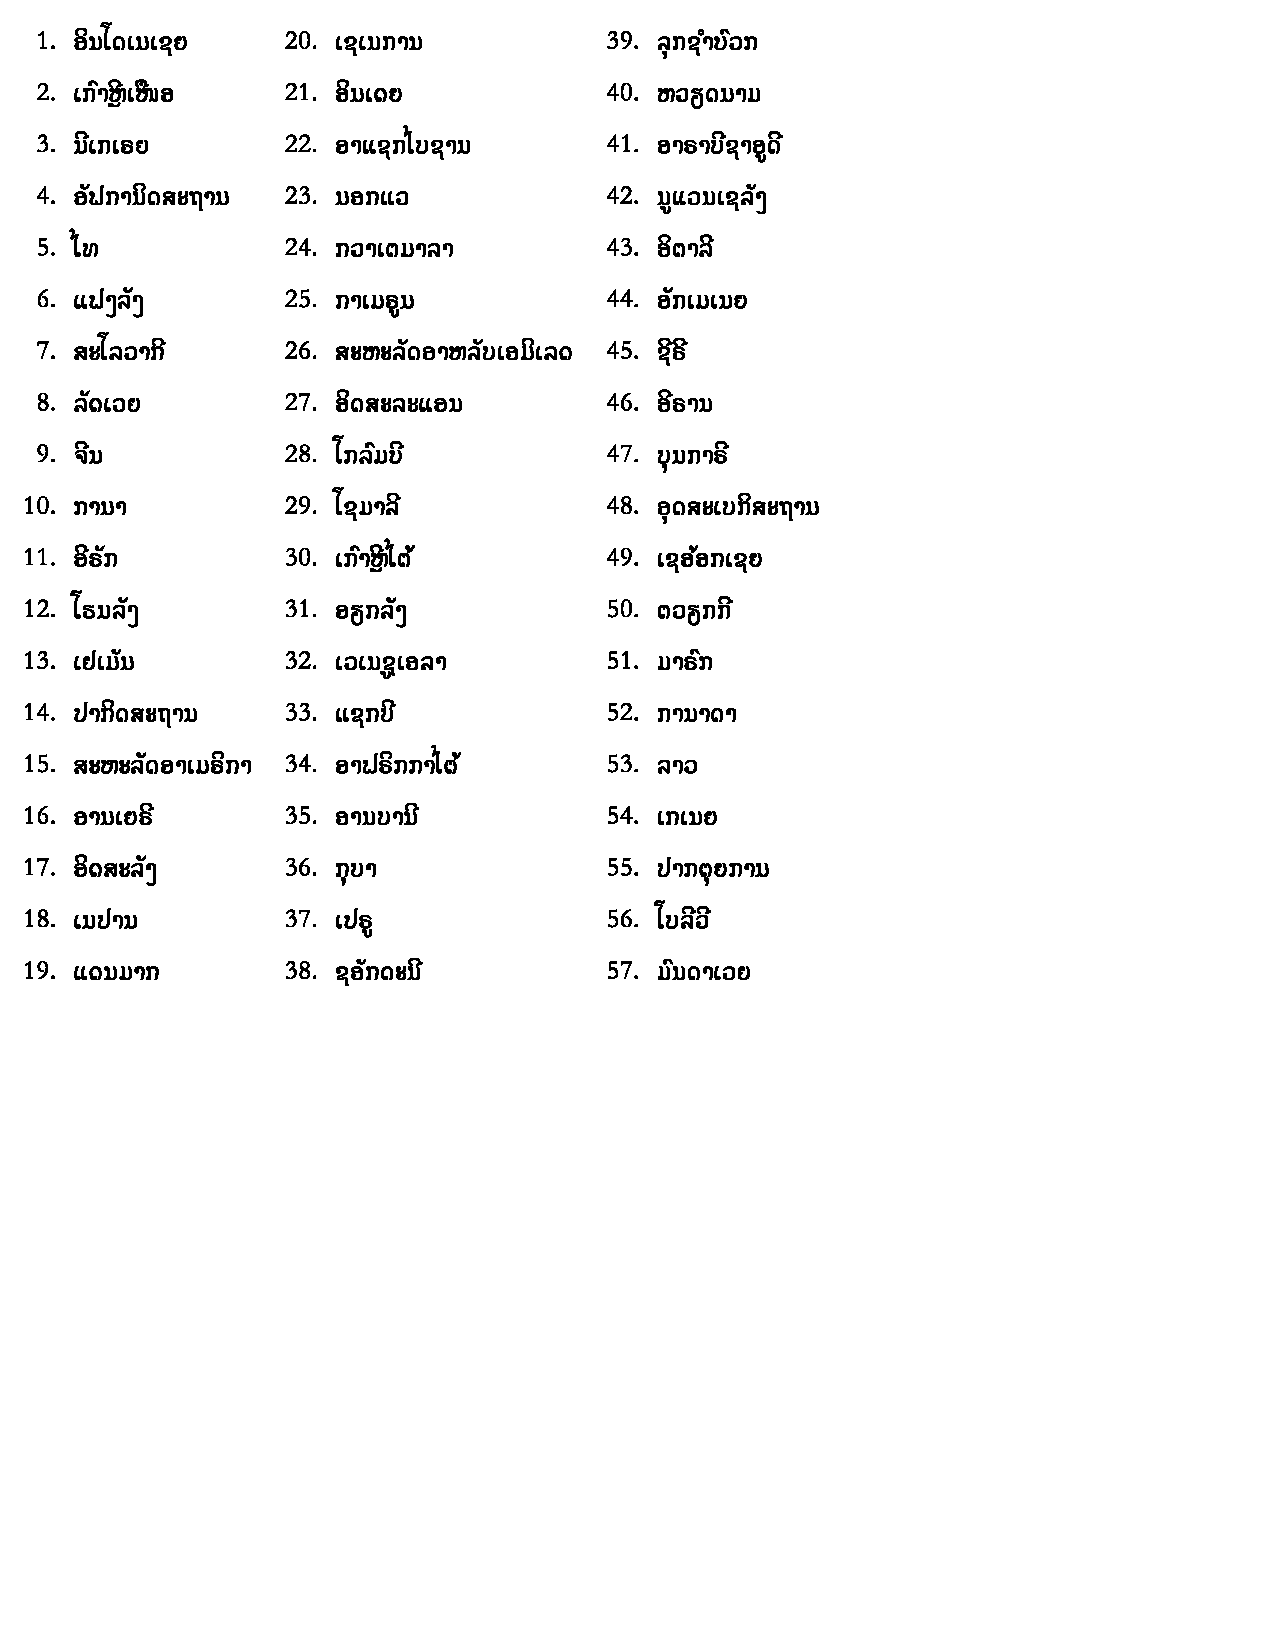
\includegraphics[bb = 0 320 500 800]{geo57Lao.pdf}}
% geo57Lao.pdf

%
\begin{assgts}
\item \findland.
\item \guessond.
\end{assgts}
%
\by{—\BIname}

\makepart{\respsing {\teamcont}}
%\makepart{\solusing {\teamcont}}
%\thispagestyle{empty}
\pagestyle{somestyle}

\centerline{\begin{tabular}{r\lr l}
\georow{1}{indōnēsiya}{\idLand}\\
\georow{2}{kaw{\super h}ḷī {\super h}n\={ʉ}a}{\kpLand}\\
\georow{3}{nīkēliya}{\ngLand}\\
\georow{4}{âfkānitsatʰān}{\afLand}\\
\georow{5}{tʰai}{\thLand}\\
\georow{6}{fǣṅlâṅ}{\fiLand}\\
\georow{7}{salōvākī}{\skLand}\\
\georow{8}{lâtviya}{\lvLand}\\
\georow{9}{čīn}{\cnLand}\\
\georow{10}{kānā}{\ghLand}\\
\georow{11}{īlâk}{\iqLand}\\
\georow{12}{hōnlâṅ}{\nlhLand\ \zagrad{\nlLand}}\\
\georow{13}{yēmen}{\yeLand}\\
\georow{14}{pākitsatʰān}{\pkLand}\\
\georow{15}{sahalât āmēlikā}{\usLand}\\
\georow{16}{ānñēlī}{\dzLand}\\
\georow{17}{itsalâṅ}{\isLand}\\
\georow{18}{nēpān}{\npLand}\\
\georow{19}{dǣnmāk}{\dkLand}\\
\georow{20}{sēnēkān}{\snLand}\\
\georow{21}{indiya}{\inLand}\\
\georow{22}{āsækbaisân}{\azLand}\\
\georow{23}{n\={ɔ}kvǣ}{\noLand}\\
\georow{24}{kwātēmālā}{\gtLand}\\
\georow{25}{kāmēlūn}{\cmLand}\\
\georow{26}{sahalât ā{\super h}lâp ēmilēt}{\aeLand}\\
\georow{27}{itsala'ǣn}{\ilLand}\\
\georow{28}{kōlômbī}{\coLand}\\
\georow{29}{sōmālī}{\soLand}\\
\end{tabular}
\begin{tabular}{r\lr l}
\georow{30}{kaw{\super h}ḷī tái}{\krLand}\\
\georow{31}{aẏklâṅ}{\ieLand}\\
\georow{32}{vēnēsū'ēlā}{\veLand}\\
\georow{33}{sǣkbī}{\srLand}\\
\georow{34}{āflikkā tái}{\zaLand}\\
\georow{35}{ānbānī}{\alLand}\\
\georow{36}{kubā}{\cuLand}\\
\georow{37}{pēlū}{\peLand}\\
\georow{38}{sɔkdanī}{\joLand}\\
\georow{39}{luksāṃbuak}{\luLand}\\
\georow{40}{{\super h}wẏatnām}{\vnLand}\\
\georow{41}{ālābī sā'ūdī}{\saLand}\\
\georow{42}{nūvǣn ṣēlâṅ}{\nzLand}\\
\georow{43}{itālī}{\itLand}\\
\georow{44}{âkmēniya}{\amLand}\\
\georow{45}{sīlī}{\syLand}\\
\georow{46}{īlān}{\irLand}\\
\georow{47}{bunkālī}{\bgLand}\\
\georow{48}{utsabēkisatʰān}{\uzLand}\\
\georow{49}{sē'óksiya}{\geLand}\\
\georow{50}{twaẏkkī}{\trLand}\\
\georow{51}{mālôk}{\maLand}\\
\georow{52}{kānādā}{\caLand}\\
\georow{53}{lāw}{\loLand}\\
\georow{54}{kēniya}{\keLand}\\
\georow{55}{pāktuykān}{\ptLand}\\
\georow{56}{bōlīvī}{\boLand}\\
\georow{57}{môndāviya}{\mdLand}\\
\end{tabular}}

\end{document}
